\documentclass[a4paper,dvipsnames]{report}
%%%%%%%%%%%%%%%%%%%%%%%%%%%%%%%%%%%%%%%%
\usepackage{tikz}
\usepackage{float}
\usepackage{xcolor}
\usepackage{wrapfig}
\usepackage{graphics}
\usepackage{graphicx}
\usepackage{hyperref}
\usepackage{ragged2e}
\usepackage{subcaption}
\captionsetup{justification=centering}
%%%%%%%%%%%%%%%%%%%%%%%%%%%%%%%%%%%%%%%%%%%%%%%%%%%%%%%%%%%%%%%%%%%%%%%%%%%%%%%%

%%%%%%%%%%%%%%%%%%%%%%%%%%%%%%%%%%%%%%%%
% https://people.bath.ac.uk/feb/lwarp/M216-notes.tex
%% I hate indented paras
\setlength{\parindent}{0pt}
\setlength{\parskip}{6pt}
%%%%%%%%%%%%%%%%%%%%%%%%%%%%%%%%%%%%%%%%
\graphicspath{{./figs/}}
%%%%%%%%%%%%%%%%%%%%%%%%%%%%%%%%%%%%%%%%
%%%%%%%%%%%%%%%%%%%%%%%%%%%%%%%%%%%%%%%%
\setcounter{tocdepth}{1}
%%%%%%%%%%%%%%%%%%%%%%%%%%%%%%%%%%%%%%%%

%%%%%%%%%%%%%%%%%%%%%%%%%%%%%%%%%%%%%%%%%%%%%%%%%%%%%%%%%%%%%%%%%%%%%%%%%%%%%%%%
\title{Aravindh Krishnamoorthy (Personal Website)}
\date{}
\author{}
%%%%%%%%%%%%%%%%%%%%%%%%%%%%%%%%%%%%%%%%%%%%%%%%%%%%%%%%%%%%%%%%%%%%%%%%%%%%%%%%

\begin{document}
%%%%%%%%%%%%%%%%%%%%%%%%%%%%%%%%%%%%%%%%%%%%%%%%%%%%%%%%%%%%%%%%%%%%%%%%%%%%%%%%
% ================================================================================
% Title and Contents
% ================================================================================
%%%%%%%%%%%%%%%%%%%%%%%%%%%%%%%%%%%%%%%%
\maketitle
%%%%%%%%%%%%%%%%%%%%%%%%%%%%%%%%%%%%%%%%
\begin{wrapfigure}{l}{100pt}
	\begin{center}
		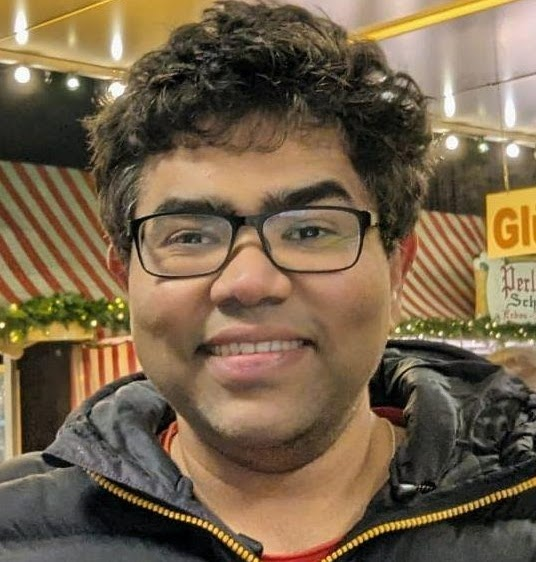
\includegraphics[width=100pt,keepaspectratio]{ark_2023.jpeg}
	\end{center}
	\caption*{(2023)}
\end{wrapfigure}
\justifying \noindent Aravindh Krishnamoorthy received his M.Sc. and Ph.D. (Dr.-Ing.) degrees from the Friedrich-Alexander University of Erlangen-Nuremberg (FAU), Germany, in 2015 and 2024, respectively, and B.E. from Visvesvaraya Technological University, India, in 2003. From 2003 to 2024, he was employed at Philips and NXP Semiconductors, Ericsson, Fraunhofer IIS, and FAU. Since 2025, he is at the LiFi Research and Development Centre, University of Cambridge, UK.	
	
Aravindh's industrial experience spans system and algorithm design for 2/4/5G communication systems, standardization, numerical and matrix analysis, digital signal processing, and embedded (vector) programming. His research areas include system and algorithm design for radio frequency and optical systems, linear algebra, and information and communication theories. Aravindh is an author of several patents and IEEE journal articles. He is also an open source programmer and an open research proponent.
	
Aravindh's doctorate was sponsored by the Fraunhofer foundation via Fraunhofer IIS.

Contact: \href{mailto:aravindh.krishnamoorthy@fau.de }{aravindh.krishnamoorthy@fau.de} (will be forwarded to the current address)

\hrulefill
%%%%%%%%%%%%%%%%%%%%%%%%%%%%%%%%%%%%%%%%%%%%%%%%%%%%%%%%%%%%%%%%%%%%%%%%%%%%%%%%
\section*{Highlights}
\begin{itemize}
	\item \href{https://aravindh-krishnamoorthy.github.io/ark-math/}{Mathematics Blog}, with a chapter on \href{https://aravindh-krishnamoorthy.github.io/ark-math/Ch4.html}{Errata for my publications}
	\item \href{https://github.com/aravindh-krishnamoorthy}{Current open source profile including pinned projects on GitHub}
\end{itemize}
\hrulefill
%%%%%%%%%%%%%%%%%%%%%%%%%%%%%%%%%%%%%%%%%%%%%%%%%%%%%%%%%%%%%%%%%%%%%%%%%%%%%%%%
\section*{Quick Links}
\begin{itemize}
	\item Research: \href{https://orcid.org/0000-0001-7186-121X}{ORCID}, \href{https://arxiv.org/a/krishnamoorthy_a_1.html}{arXiv preprints}, \href{https://ieeexplore.ieee.org/author/37086238080}{IEEE Xplore Profile}
	\item Aggregated data: \href{https://scholar.google.com/citations?user=eLf3E1kAAAAJ&hl=en}{Google Scholar}, \href{https://patents.google.com/?inventor=aravindh+krishnamoorthy}{Google Patents}, \href{http://publica.fraunhofer.de/autoren/Krishnamoorthy,%20A}{Fraunhofer Publications}
	\item Open-source programming: \href{https://github.com/aravindh-krishnamoorthy}{GitHub}, \href{https://gitlab.com/aravindh.krishnamoorthy}{GitLab}, \href{https://www.mathworks.com/matlabcentral/profile/authors/3862426}{MathWorks File Exchange}
	\item Blogging: \href{https://aravindh-krishnamoorthy.github.io/ark-math/}{Mathematics Blog}, \href{http://aravindhk.blogspot.com/}{Casual Blog}	
\end{itemize}
\hrulefill
%%%%%%%%%%%%%%%%%%%%%%%%%%%%%%%%%%%%%%%%%%%%%%%%%%%%%%%%%%%%%%%%%%%%%%%%%%%%%%%%
\section*{Work Experience}
\begin{itemize}
	\item 2G/4G/5G communication systems design
	\item Algorithm design including filters and sample rate converters
	\item Linear algebra, numerical analysis, error analysis
	\item Vectorisation, hardware/software partitioning, fixed/floating point designs, timing analysis, system dimensioning, standardization
	\item 15+ patents in communication systems
\end{itemize}
\hrulefill
%%%%%%%%%%%%%%%%%%%%%%%%%%%%%%%%%%%%%%%%%%%%%%%%%%%%%%%%%%%%%%%%%%%%%%%%%%%%%%%%
\section*{Research Experience}
\begin{itemize}
	\item Free-space optical communication [\href{https://ieeexplore.ieee.org/abstract/document/10974735}{IEEE Xplore}]
	\item 5/6G algorithms: Non-orthogonal and linear precoding and decoding, massive MIMO [\href{https://open.fau.de/handle/openfau/31976}{Cumulative Thesis}]. Cumulative thesis contains all major publications
	\item Joint papers with students: (2019) M. Goodarzi \href{https://ieeexplore.ieee.org/abstract/document/8661311}{IEEE Xplore}, (2021) M. Huang \href{https://doi.org/10.1109/WCNC49053.2021.9417424}{IEEE Xplore}, (2022) R. Diab \href{https://ieeexplore.ieee.org/document/9814475}{IEEE Xplore}.
	\item \href{https://www.iis.fraunhofer.de/en/ff/kom/mobile-kom/sudas.html}{SUDAS}
\end{itemize}
Note: All research papers are also available on \href{https://arxiv.org/a/krishnamoorthy_a_1.html}{arXiv}.

\hrulefill
%%%%%%%%%%%%%%%%%%%%%%%%%%%%%%%%%%%%%%%%%%%%%%%%%%%%%%%%%%%%%%%%%%%%%%%%%%%%%%%%
\section*{Personal Life}
\begin{itemize}
	\item Hobbies: Hiking, biking, rally racing, winter swimming, competitive mathematics
	\item Meritorious with $> 99.5$ percentile in several national and international competitive exams since childhood
	\item Numerous awards and scholarships during studies
	\item Recognized contributions to several open source software
\end{itemize}
\hrulefill
%%%%%%%%%%%%%%%%%%%%%%%%%%%%%%%%%%%%%%%%%%%%%%%%%%%%%%%%%%%%%%%%%%%%%%%%%%%%%%%%
\begin{center}
	Copyright (C) 2025 - present, Aravindh Krishnamoorthy, contact via university e-mail address given on the top of the page.
\end{center}
%%%%%%%%%%%%%%%%%%%%%%%%%%%%%%%%%%%%%%%%%%%%%%%%%%%%%%%%%%%%%%%%%%%%%%%%%%%%%%%%
\end{document}
